\documentclass[11pt,a4paper,openany,leqno]{article}

\textwidth=160mm \textheight=260mm \hoffset=-18mm \voffset=-30mm
\setcounter{page}{1}
			\usepackage[magyar]{babel}
			\usepackage[utf8]{inputenc}
			\usepackage[T1]{fontenc}
			\usepackage{indentfirst}
			\usepackage{amsmath,esint}
			\usepackage{amssymb}
%			\usepackage{eufrak}
			\usepackage{psfrag}
			\usepackage{tabularx}
			\usepackage{graphicx}
			\usepackage{wrapfig}	
			\usepackage{hyperref}
			\usepackage{multicol}	
									
			\frenchspacing
			\allowhyphens

\tolerance=2000
\hbadness=2000
\vbadness=10000
\overfullrule=0pt




\begin{document}
\section{Indukció I.}
\subsection{Kovács-Párkányi Fizikai Példatár II. / 470.feladat}


 \indent
Egy $a$ és $b$ oldalú téglalap alakú vezetőkeret egy síkban fekszik a végtelen hosszú egyenes vezetővel, amelyben $I$ erősségű áram folyik. A vezető a $b$ oldallal párhuzamos és $d>a$ távolságra van a leközelebbi oldaltól. Mekkora $Q$ elektromos töltésmennyiség halad keresztül a keret tetszés szerinti vezető keresztmetszetén, ha a keret a vezetőköz közelebbi $b$ oldal körül $180 ^{\circ} $-kal elfordul, s ebben a helyzetben marad? A keret vezetékének keresztmetszete $A$, fajlagos ellenállása $\varrho$.

\begin{figure}[h!]
\centering
  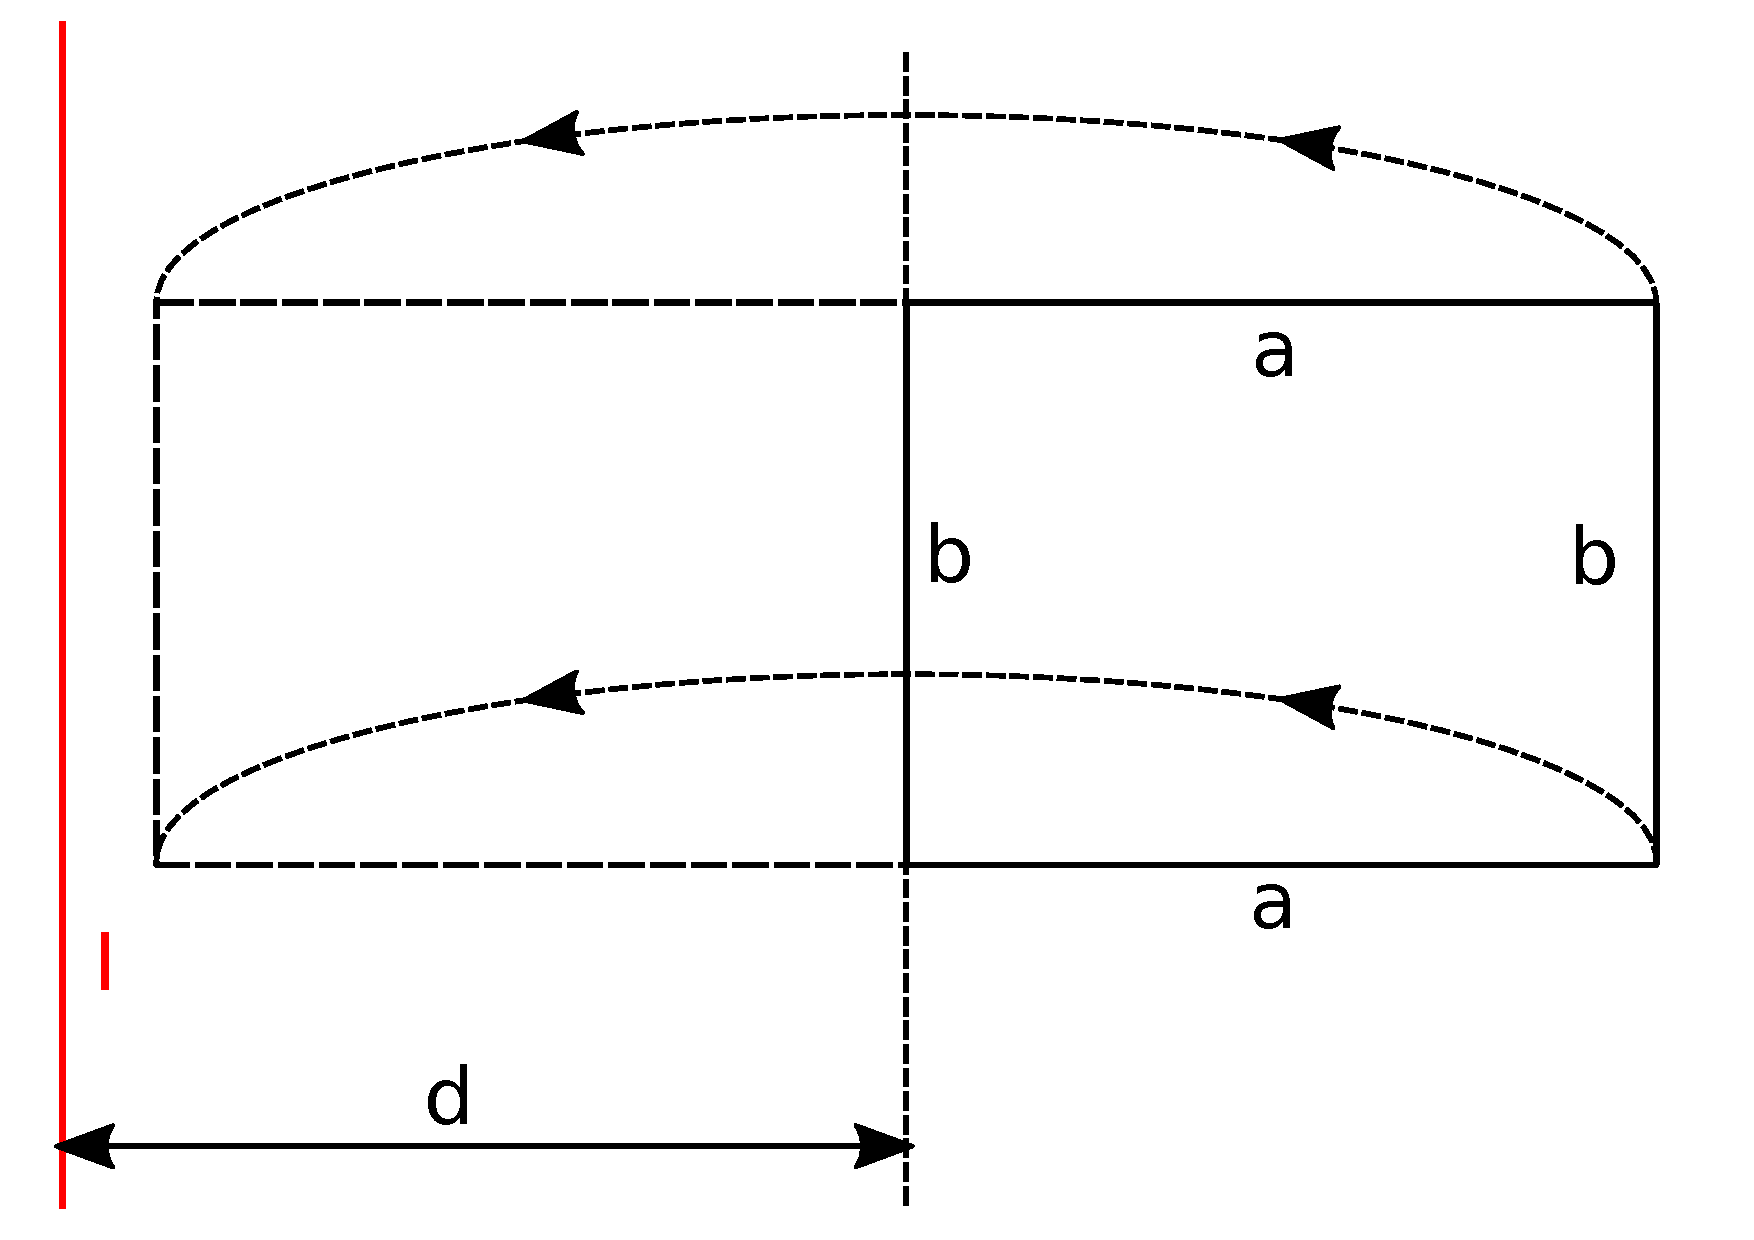
\includegraphics[width=100mm,scale=0.5]{kep1.pdf}
  \caption{A vezetőkeret forgása és a végtelen hosszú huzal}
  \label{}
\end{figure} 


\begin{flushright} {Feladatot kidolgozta: {\it Z2R8XS}} \end{flushright}

\vspace{0.5cm}

\textbf{Megoldás}\\
\indent
Válasszunk koordinátarendszert, és legyen a végtelen hosszú vezetőben folyó áram jele $I$ helyett $I_0$. A vezetőkeretben elinduló áram jele legyen $I$ - ez függni fog a keret pozicíójától.\\ 
\begin{figure}[h!]
\centering
  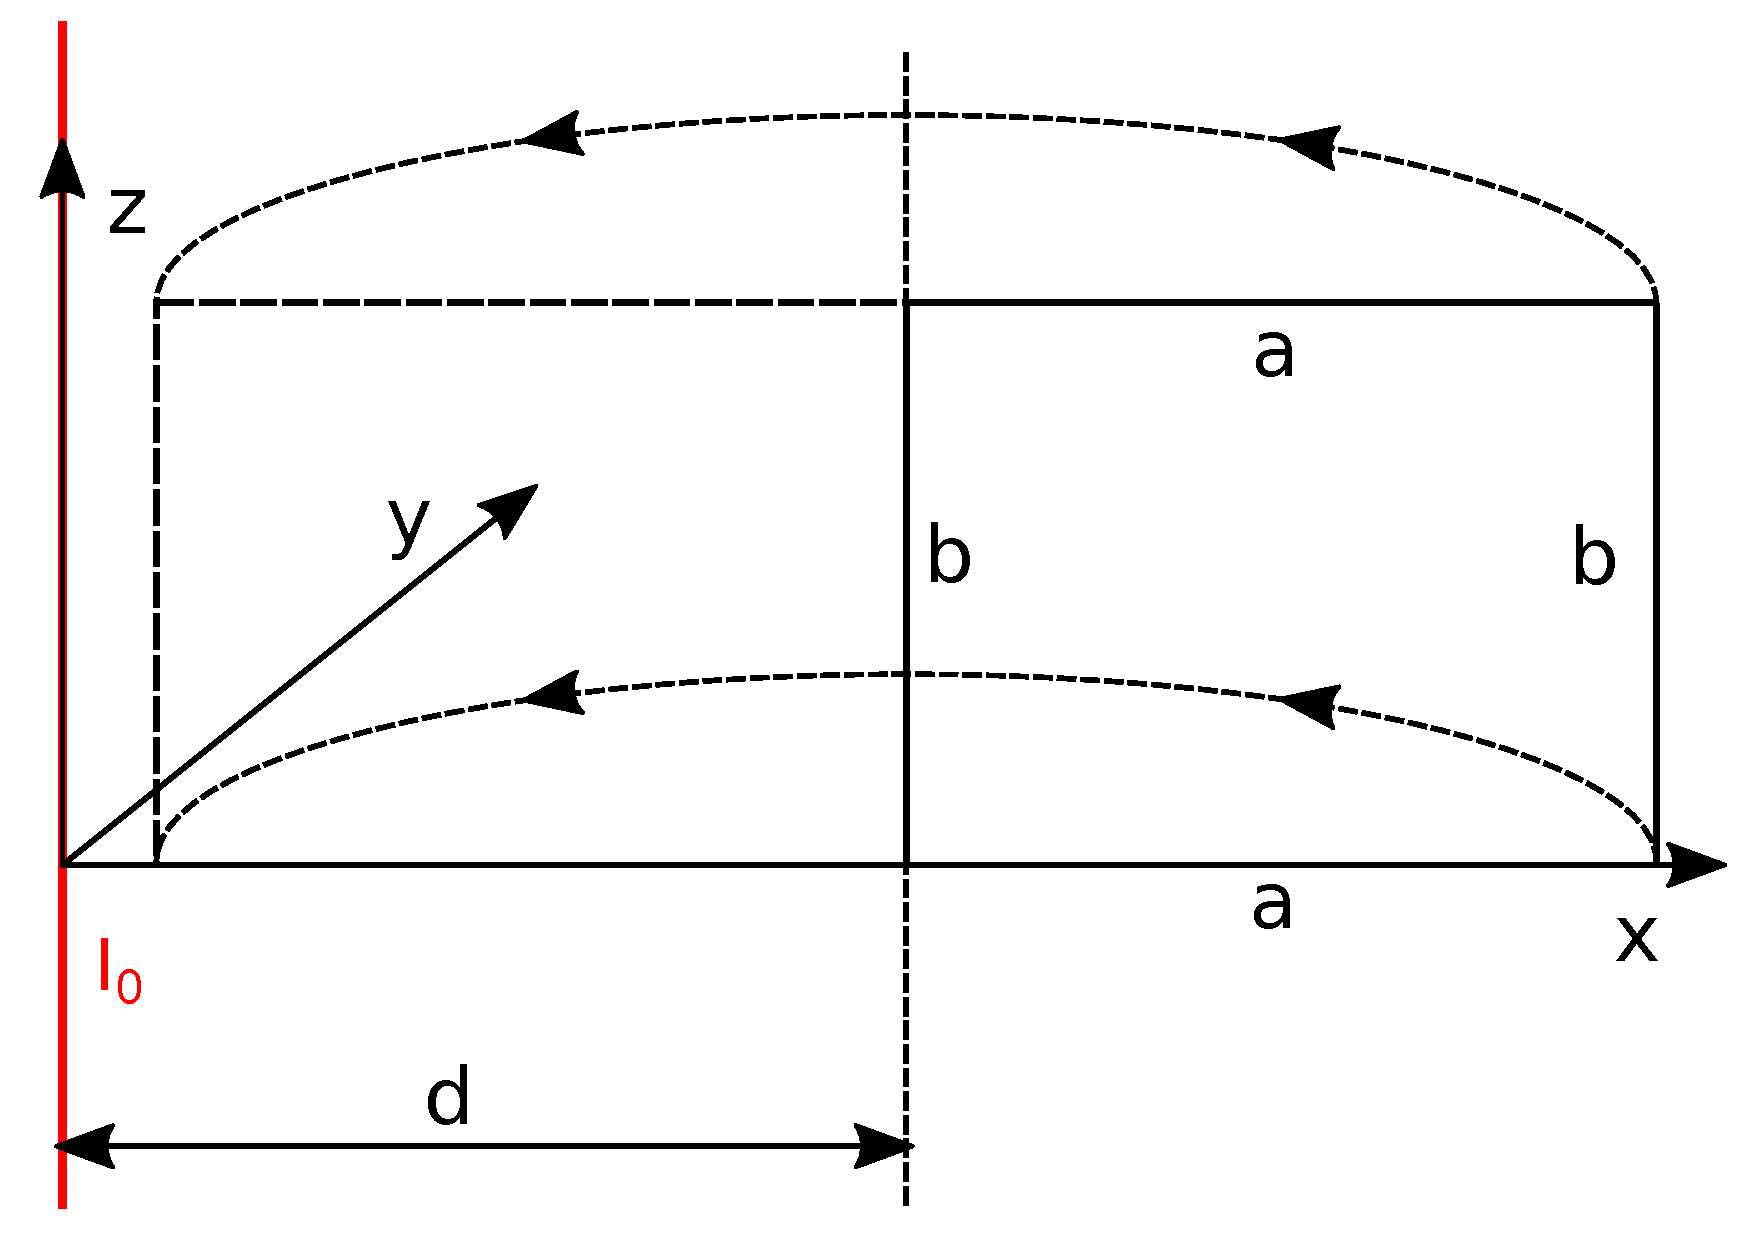
\includegraphics[width=100mm,scale=0.5]{kep2.pdf}
  \caption{Koordinátarendszer választása}
  \label{}
\end{figure} \\ \\
\indent 
Tudjuk, hogy az indukált feszültség egy egyenes vezetőre\\ 
$$ U_i = \vec{l} (\vec{v}\times\vec{B}) $$ \indent

Először vizsgáljuk meg, milyen lesz a $z$ tengelyre merőleges, $a$ hosszúságú vezetőkben az indukált feszültség. Egy kis $\Delta \vec{l}$ vezetődarabkában $\Delta U_i$ feszültség fog ébredni az ottani $\vec{B}$ mágneses tér hatására, ha a $\Delta \vec{l}$-nek egy $\vec{v}$ sebessége van.

\begin{itemize}
  \item Látható, hogy a kis huzaldarabkát jellemző $\Delta \vec{l}$ vektornak nem lesz $z$ komponense, bárhol is vagyunk bármelyik $a$ oldalon.
  \item Ha rögzítenénk a forgástengelyhez egy polárkoordinátarendszert, mely párhuzamos az $(x,y)$ síkkal, és felírnánk a $\vec{v}$ sebességet, akkor csak $\phi$ irányú komponense lenne, radiálisan és felfelé nem mozdul el egyik oldal sem. Állítható, hogy $\vec{v}$-nek sem lesz $z$ komponense. 
  \item A végtelen hosszú áramjárta huzal által keltett mágneses tér vektora hasonló analógiával úgyszint "$\phi$" irányú, ha vezeterőre rögzítenénk egy $(x,y)$ síkkal párhuzamos polárkoordinátarendszert. A $\vec{B}$ vektornak sem lesz $z$ komponense.
\end{itemize} 


Az $U_i$-vel egyenlő kifejezés egy vegyes szorzat. Egy vegyes szorzat a három vektor által kifeszített test térfogatát adja meg. E három vektor esetünkben egy síkban van, az $(x,y)$ síkban. Komplanáris vektorok által kifeszített paralelepipedon térfogata $0$.\\ 
\indent
Mindezek alapján az állítás az, hogy a keret $z$ tengelyre merőleges oldalainak nem lesz járuléka - a keretben ébredő áram szempontjából.\\
\indent
A forgástengelyen lévő $b$ hosszúságú oldalnak úgyszint nem lesz járuléka, mert nem is fog elmozdulni.\\ 
\indent 
A kezdetben a vezetőtől távolabbi $b$ hosszúságú oldalnak lehet csak járuléka. Itt minden $\Delta \vec{l}$ darabkának csak $z$ komponense van, míg $\vec{v}$ és $\vec{B}$ minden darabka esetén az $(x,y)$ síkban van. Sőt, a mágneses térnek szimmetriája a $z$ irányú eltolás, tehát minden darabkára ugyanolyan irányú és ugyanolyan nagyságú lesz $\vec{B}$. Tekintsük merev testnek a keretet, így minden huzal darabka sebessége azonos irányú és nagyságú lesz minden időpillanatban. Ha a vezető rá merőleges tengely körül forogna, akkor az egyes pontjainak más lenne a sebessége, de mivel nem forog, működik a
$$ U_i = \vec{l} (\vec{v}\times\vec{B}) $$

képlet. Skalár lesz a vegyes szorzat értéke, mely kifejezhető a vektorok komponenseivel. Írjuk fel a vektorokat.
\begin{figure}[h!]
\centering
  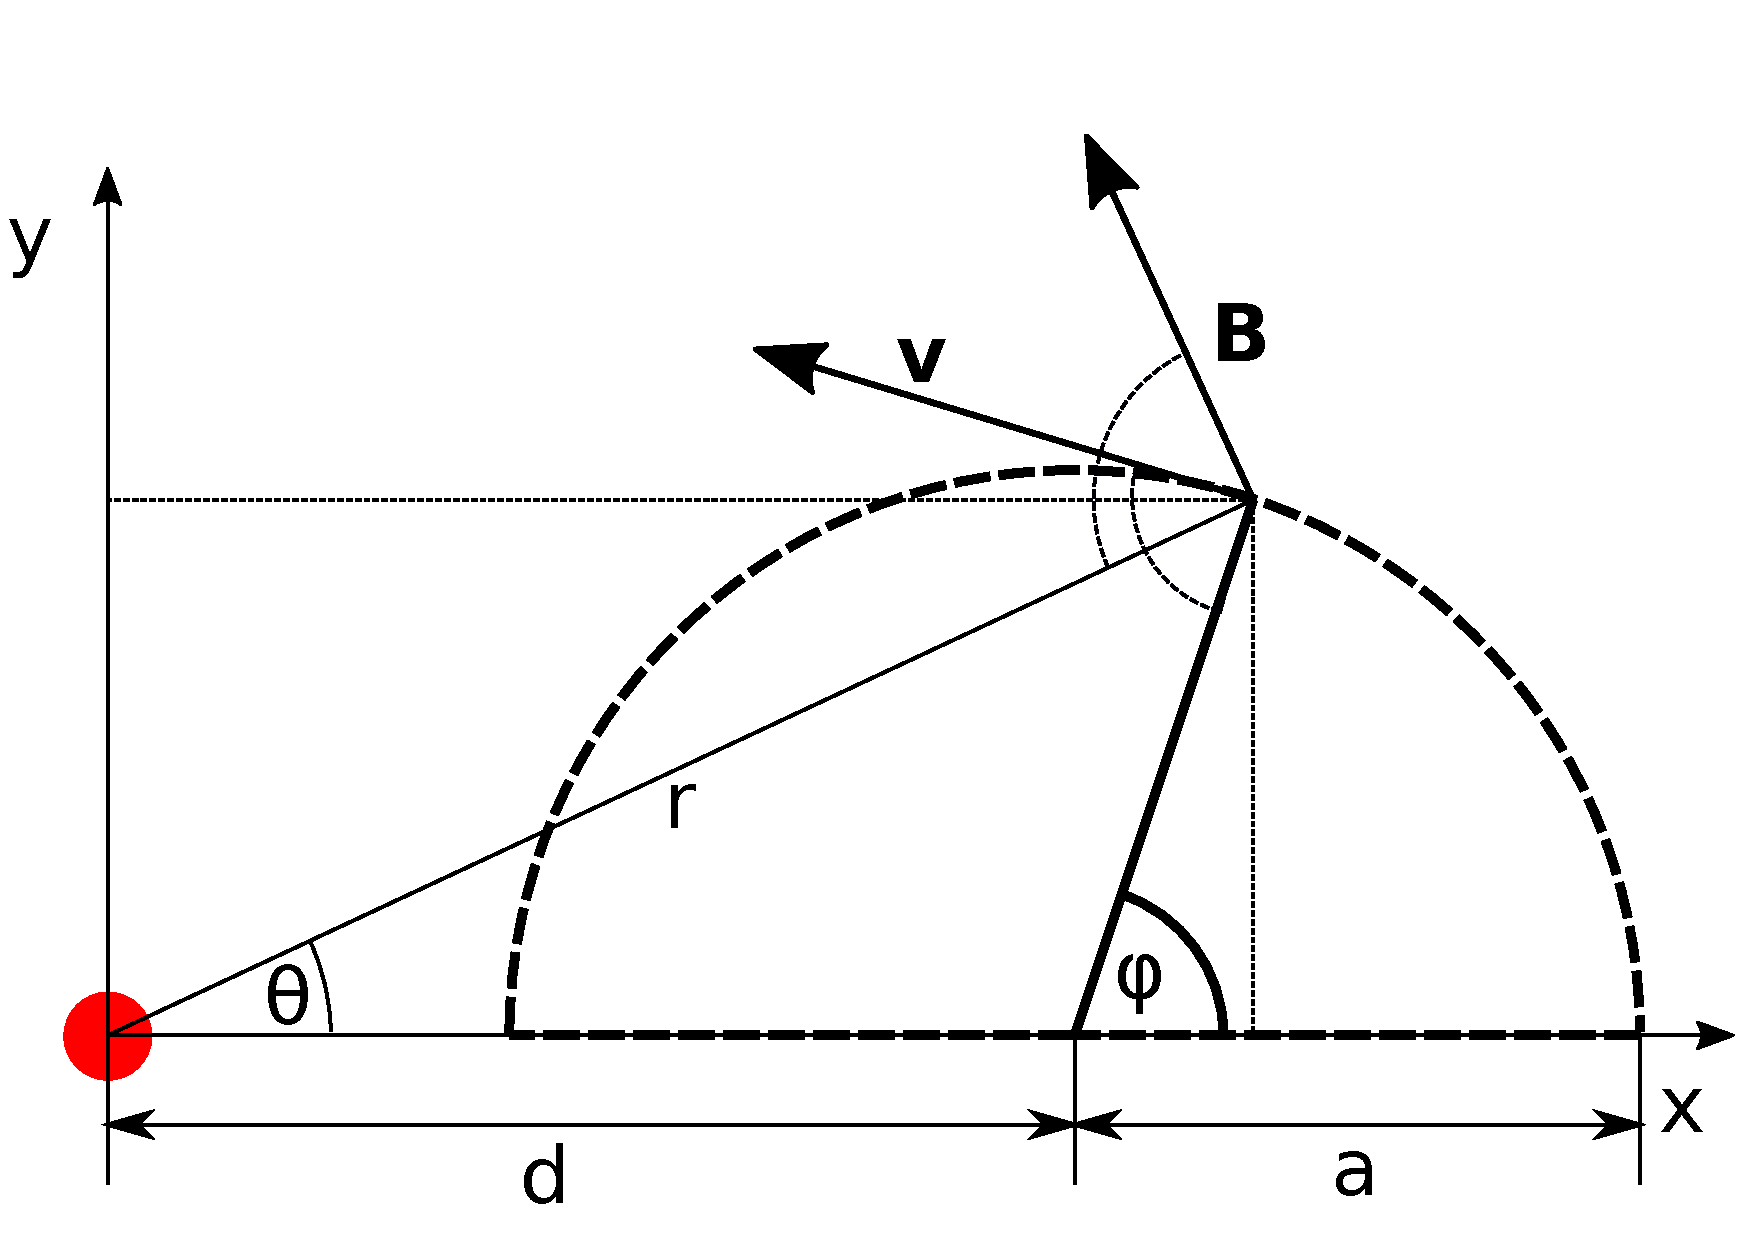
\includegraphics[width=100mm,scale=0.5]{kep3.pdf}
  \caption{A vezetőkeret és a végtelen hosszú huzal felülnézetből}
  \label{}
\end{figure}\\ \indent
Tudjuk, hogy $\vec{l}$-nek csak $z$ komponense van, és hossza $b$, így \\
$$ \vec{l} = \begin{pmatrix} 0 \\ 0 \\ b \end{pmatrix}$$ \indent
Tételezzük fel, hogy $\phi = 0$-tól $\phi=\pi$-ig konstans $\omega$ szögsebességgel fordul el a keret. Ekkor a forgó függőleges oldal pozíciója felülnézetből \\
$$ \vec{r} = \begin{pmatrix} d + a \cdot cos(\phi(t)) \\ a \cdot sin(\phi(t)) \end{pmatrix}$$\indent
Ha $\phi(t) = \omega \cdot t$, akkor
$$ \vec{v} = \begin{pmatrix} - a \cdot \omega \cdot sin(\omega\cdot t) \\ a\cdot \omega \cdot cos(\omega \cdot t) \end{pmatrix} $$\indent
A forgó függőleges oldal minden pontjának konstans a $z$ koordinátája, így a sebességnek $0$ lesz a $z$ komponense - ez releváns, mivel a vektoriális szorzást három dimenzióban kell elvégezni.\\ \indent
Tudjuk, hogy az egyenes, végtelen hosszú áramjárta vezeték által keltett mágneses tér nagysága
$$ B(r) = \frac{\mu_0}{2\pi}\cdot \frac{I_0}{r} $$
ahol $r$ a vezetőtől lévő távolság.\\ \indent
Pozitív és negatív $z$ irányba folyhat az áram. A vezetőkeretben ébredt feszültség előjele, azaz a benne folyó áram iránya függ ettől. Ezért nem rajzoltam be az előző ábárkon $I_0$ irányát. Számoljunk egyelőre úgy, hogy pozitív $z$ irányba folyik az áram. Ha negatív irányba folyna, akkor csak egy előjellel különbözne a számolás - és ez az előjel mindvégig megmaradna, egészen a $Q$ értékig. $Q$ nagyságának meghatározásánál nem játszik kulcsfontosságú szerepet, melyik irányba folyik az áram.\\ \indent
Felfelé folyó áram esetén felülnézetből a mágneses tér vektora:\\
$$ \vec{B} = \begin{pmatrix} - r \cdot sin(\Theta) \\ r \cdot cos(\Theta) \end{pmatrix} \frac{\mu_0}{2\pi}\cdot \frac{I_0}{r^2} $$ \indent
Mivel $\vec{B}$ nagysága fordítottan arányos $r$-rel. Ha kiegészítjük három dimenzióra, a fent leírtak alapján $\vec{B}$-nek $z$ komponense $0$.\\ \indent
Tehát az indukált feszültség:\\
$$ U_i = \begin{pmatrix} 0 \\ 0 \\ b \end{pmatrix} \cdot ( \begin{pmatrix} - a \cdot \omega \cdot sin(\omega\cdot t) \\ a\cdot \omega \cdot cos(\omega \cdot t) \\ 0 \end{pmatrix} \times \begin{pmatrix} - r \cdot sin(\Theta) \\ r \cdot cos(\Theta)\\0 \end{pmatrix} \frac{\mu_0}{2\pi}\cdot \frac{I_0}{r^2} ) $$

$$ U_i = \frac{\omega \cdot b \cdot\mu_0\cdot I_0}{2\pi}\cdot \frac{1}{r^2}\begin{pmatrix} 0 \\ 0 \\ 1 \end{pmatrix} \cdot ( \begin{pmatrix} - a \cdot sin(\omega\cdot t) \\ a \cdot cos(\omega \cdot t) \\0\end{pmatrix} \times \begin{pmatrix} - r \cdot sin(\Theta) \\ r \cdot cos(\Theta) \\ 0\end{pmatrix} ) $$
$$ U_i = \frac{\omega \cdot b \cdot\mu_0\cdot I_0}{2\pi}\cdot \frac{1}{r^2} (- a \cdot sin(\omega\cdot t) \cdot r \cdot cos(\Theta) - a \cdot cos(\omega \cdot t) \cdot r \cdot sin(\Theta)) $$
 $$ U_i = \frac{\omega \cdot b \cdot\mu_0\cdot I_0}{2\pi}\cdot \frac{1}{r^2} (- a \cdot sin(\phi) \cdot r \cdot cos(\Theta)- a \cdot cos(\phi) \cdot (-r \cdot sin(\Theta))) $$\indent
A geometriai összefüggések segítségével egyszerűsíteni lehet ezen a kifejezésen - a pontozott vonalak segítségünkre válthatnak. Az alábbi azonosságok alkalmazhatók.\\
$$ r^2 = (a \cdot sin(\phi))^2 + (d+a\cdot cos(\phi))^2 = a^2 + d^2 + 2a\cdot d \cdot cos(\phi)$$
$$ a \cdot sin(\phi) = r \cdot sin(\Theta) $$ 
$$ a \cdot cos(\phi) = r \cdot cos(\Theta) - d $$\indent
Ezeket behelyettesítve:\\
$$ U_i = \frac{\omega \cdot b \cdot\mu_0\cdot I_0}{2\pi}\cdot \frac{1}{a^2 + d^2 + 2a\cdot d \cdot cos(\phi)} (- a \cdot sin(\phi) (a \cdot cos(\phi) +d) + a \cdot cos(\phi) \cdot a \cdot sin(\phi)) $$
 $$ U_i = \frac{\omega \cdot b \cdot\mu_0\cdot I_0}{2\pi}\cdot \frac{-a\cdot d \cdot sin(\phi)}{a^2 + d^2 + 2a\cdot d \cdot cos(\phi)} $$\\ \indent
Az indukált feszültségre, a vezetőkeretben folyó áramra és a vezetőkeret össz ellenállására:\\
$$ U_i = I \cdot R $$
$$ I = \frac{U_i}{R} $$\indent
Ha tudjuk a vezetőkeret $\varrho$ fajlagos ellenállását, akkor az egész keret ellenállása:\\
$$ R = \frac{2 \varrho}{A}(a+b) $$\indent
Így az áram erőssége:\\
$$ I = \frac{\omega \cdot b \cdot\mu_0\cdot I_0}{2\pi}\cdot \frac{-a\cdot d \cdot sin(\phi)}{a^2 + d^2 + 2a\cdot d \cdot cos(\phi)}\frac{A}{2 \varrho (a+b)} $$
$$ I = \frac{\omega \cdot b \cdot\mu_0\cdot I_0\cdot A}{8\pi \varrho (a+b)}\cdot \frac{-2a\cdot d \cdot sin(\phi)}{a^2 + d^2 + 2a\cdot d \cdot cos(\phi)} $$
$$ I = \frac{\omega \cdot b \cdot\mu_0\cdot I_0\cdot A}{8\pi \varrho (a+b)}\cdot \frac{-2a\cdot d \cdot sin(\omega \cdot t)}{a^2 + d^2 + 2a\cdot d \cdot cos(\omega \cdot t)} $$\indent
Tudjuk, hogy a vezető keresztmetszetén áthaladó töltésmennyiség idő szerinti deriváltja az áramerősség. Megkaptuk az áramerősséget, ebből visszaintegrálható az áthaladt töltésmennyiség $t_0$ és $t_1$ időpontok között, amennyiben $t_0$ pillanatban kezdődött a forgás és $t_1$ pillanatban fejeződött. Legyen $t_0 = 0$, így $\phi(0) = 0$. Legyen $t_1 = \pi / \omega$, így $\phi(t_1) = \pi $. Az időtől nem függő mennyiségek kiemelhetők az integrálás elé. \\
$$ Q = \frac{\omega \cdot b \cdot\mu_0\cdot I_0\cdot A}{8\pi \varrho (a+b)} \int_{0}^{\pi/\omega} \cdot \frac{-2a\cdot d \cdot sin(\omega \cdot t)}{a^2 + d^2 + 2a\cdot d \cdot cos(\omega \cdot t)} dt $$\indent
Egy hasznos azonosság integrálásra:\\
$$ \int\frac{f'(x)}{f(x)}dx = ln|f(x)| + c $$\indent
Most a $+c$ konstanssal nem kell foglalkozni, mivel határozott integrál esetén ki fog esni.\\
$$ Q = \frac{\omega \cdot b \cdot\mu_0\cdot I_0\cdot A}{8\pi \varrho (a+b)} [ln(a^2 + d^2 + 2a\cdot d \cdot cos(\omega \cdot t))]_0^{\pi/\omega} $$
$$ Q = \frac{\omega \cdot b \cdot\mu_0\cdot I_0\cdot A}{8\pi \varrho (a+b)} [ln(a^2 + d^2 + 2a\cdot d \cdot cos(\pi)) - ln(a^2 + d^2 + 2a\cdot d \cdot cos(0))] $$
$$ Q = \frac{\omega \cdot b \cdot\mu_0\cdot I_0\cdot A}{8\pi \varrho (a+b)} [ln((a-d)^2) - ln((a+d)^2)] $$
$$ Q = \frac{\omega \cdot b \cdot\mu_0\cdot I_0\cdot A}{8\pi \varrho (a+b)} ln((\frac{a-d}{a+d})^2) $$ \indent
Tehát $ Q = \frac{\omega \cdot b \cdot\mu_0\cdot I_0\cdot A}{8\pi \varrho (a+b)} ln((\frac{a-d}{a+d})^2) $ elektromos töltésmennyiség halad keresztül a keret tetszés szerinti keresztmetszetén.






\end{document}